\documentclass[11pt, a4paper, norsk]{NTNUoving}
\usepackage[utf8]{inputenc}
\usepackage[T1]{fontenc}
\usepackage{mathrsfs}
\newcommand{\RomanNumeralCaps}[1]
{\MakeUppercase{\romannumeral #1}}


\ovingnr{7}    % Nummer på innlevering
\semester{Haust 2022}
\fag{TMA4120}
\institutt{Institutt for matematiske fag}

\begin{document}
\section*{13.1}
\begin{oppgave}[2]
  Plotter de komplekse tallene, og ser at de korresponderende fargene har rett vinkel mellom seg.
  \[
    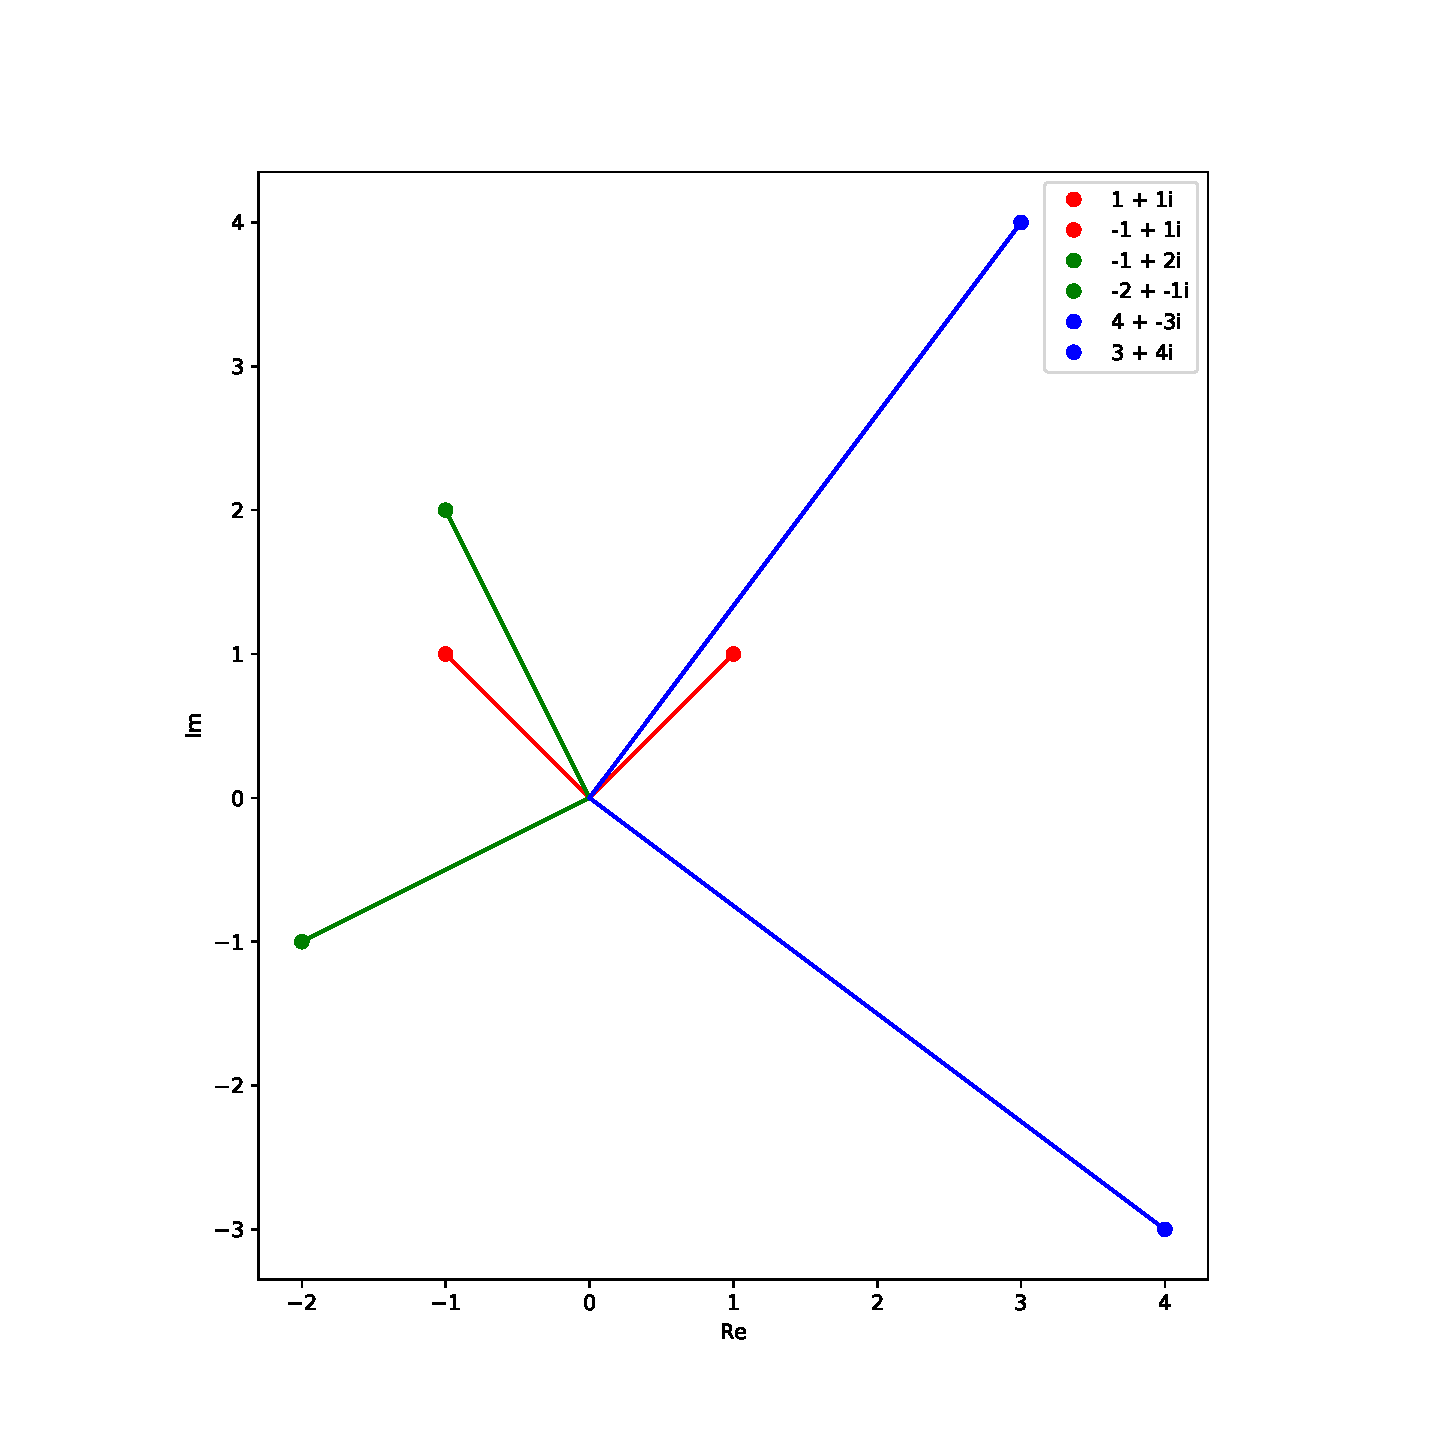
\includegraphics[scale=0.4]{13.1.2.pdf}
  \]
\end{oppgave}
\begin{oppgave}[3]
  Bruker teknikken i $(7)$.
  \begin{align*}
    \frac{26-18i}{6-2i} &= \frac{(13-9i)(3+i)}{(3-i)(3+i)}\\
                        &= \frac{39-27i+13i+9}{10} \\
                        &= \frac{24}{5}-\frac{7}{5}i
  \end{align*}
  Ved å bruke formelen i $(7)$ blir svaret
  \begin{align*}
    z &= \frac{x_1x_2+y_1y_2}{x_2^2+y_2^2} + i\frac{x_2y_1+x_1y_2}{x_2^2+y_2^2}\\
    &=  \frac{26\cdot 6+(-18)\cdot (-2)}{6^2+(-2)^2} + 
    i\frac{6\cdot (-18)-26\cdot (-2)}{6^2+(-2)^2}\\ 
    &= \frac{24}{5}-\frac{7}{5}i
  \end{align*}  
\end{oppgave}
\begin{oppgave}[14]
  Har $z_1=-2+5i$ og $z_2=3-i$. Det gir
  \begin{align*}
    \frac{\overline{z_1}}{\overline{z_2}} &= \frac{-2-5i}{3+i} \\
                                &= \frac{-(2+5i)(3-i)}{(3+i)(3-i)} \\
                                &= \frac{-6+2i-15i-5}{9+1} \\
                                &= -\frac{11}{10} - \frac{13}{10} i 
  \end{align*}
  og
  \begin{align*}
    \frac{z_1}{z_2} &= \frac{-2+5i}{3-i} \\
                               &= \frac{(-2+5i)(3+i)}{(3-i)(3+i)} \\
                               &= \frac{-6-2i+15i-5}{9+1} \\
                               &= \frac{-11+13i}{10} \\
    \Rightarrow \overline{\frac{z_1}{z_2}} &= -\frac{11}{10}-\frac{13}{10}i \\
  \end{align*}
\end{oppgave}  
\begin{oppgave}[16]
  Begynner med å løse brøkene gitt $z=x+iy$.
  \[
    \frac{1}{x+iy} = \frac{x}{x^2+y^2}-\frac{y}{x^2+y^2}i
  \]  
  Dermed er
  \[
    \text{Im}(1/z)=-\frac{y}{x^2+y^2}
  \]
  Tilsvarende blir
  \[
    \frac{1}{(x+iy)^2}=\frac{1}{(x^2-y^2)+i2xy}=\frac{(x^2-y^2)-i2xy}{(x^2-y^2)^2+4x^2y^2}=\frac{(x^2-y^2)-i2xy}{(x^2+y^2)^2}
  \]
  og
  \[
    \text{Im}(1/z^2)=\frac{2xy}{(x^2+y^2)^2}
  \]  
\end{oppgave}  
\newpage
\section*{13.2}
\begin{oppgave}[1]
Har $z=1+i$. Det gir
\begin{align*}
  \theta &= \text{Arg}(z)=\arctan(1)=\pi/4\\
  r &= \text{Abs}(z)=\sqrt{1^2+1^2}=\sqrt{2}
\end{align*}
som betyr at
\[
  z=re^{i\theta}=\sqrt{2}e^{i\pi/4}
\]
\end{oppgave}
\begin{oppgave}[8]
  Begynner med å dele brøken opp i reell og imaginær del.
  \begin{align*}
    \frac{7+4i}{3-2i} &= \frac{(7+4i)(3+2i)}{3^2+2^2} \\
                      &= \frac{21 + 14i+12i -8}{13} \\
                      &= 1 + 2i
  \end{align*}
  Dette gir
  \[
    z=\sqrt{5}e^{i\arctan{2}}
  \]  
\end{oppgave}
\begin{oppgave}[11]
  Har $z=\sqrt{3}\pm i$, som gir
  \[
    \text{Arg}(z)=\arctan\frac{\pm 1}{\sqrt{3}} = \pm \frac{\pi}{6}
  \]
  Slik ser det ut i det komplekse plan:
  \[
    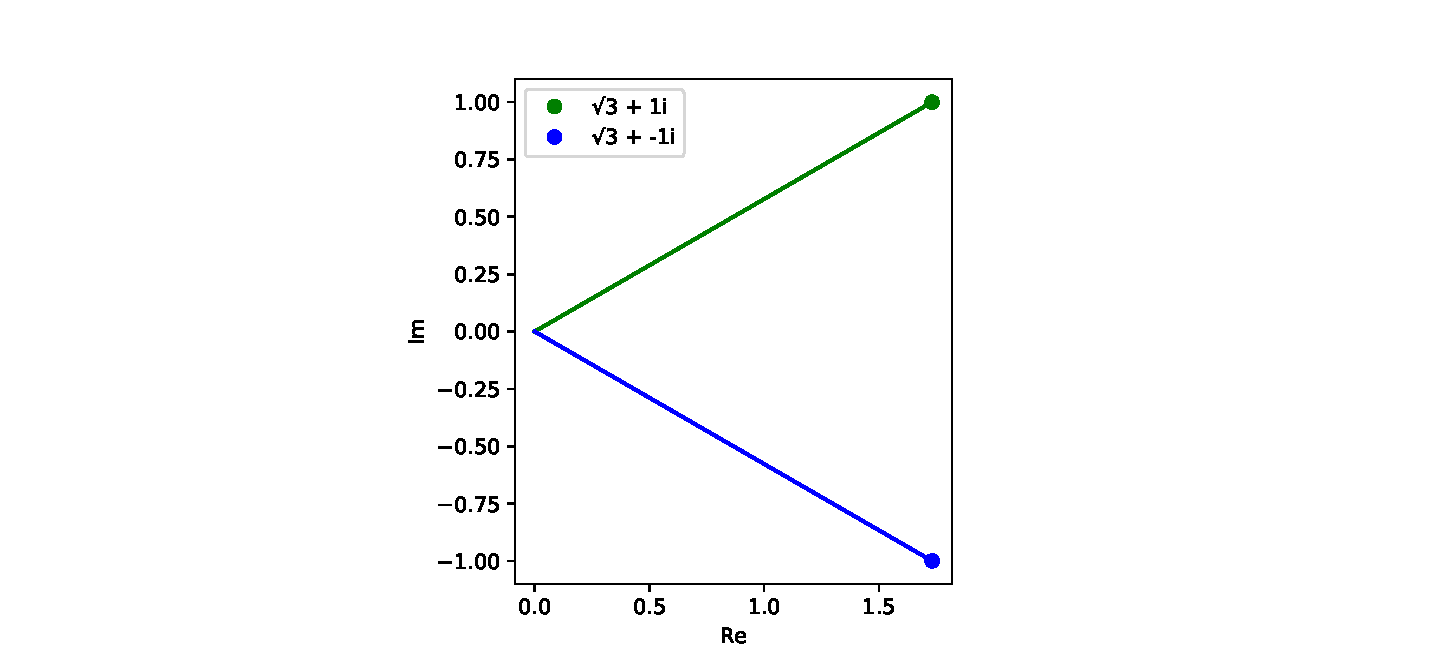
\includegraphics[scale=0.6]{13.2.11.pdf}
  \]
\end{oppgave}
\begin{oppgave}[21]
  Finner først $z=1-i$ på polar form.
  \[
    z = \sqrt{2}e^{-i\pi/4}
  \]
  Ved De Moivres formel finner vi tredjerøttene
  \[
    \sqrt[3]{1-i} = \sqrt[6]{2}\exp \left[\left(-\frac{\pi}{12}+\frac{2\pi k}{3}\right)i\right], k\in\{0, 1, 2\}
  \]
  Kan plotte disse røttene i det komplekse plan:
  \[
    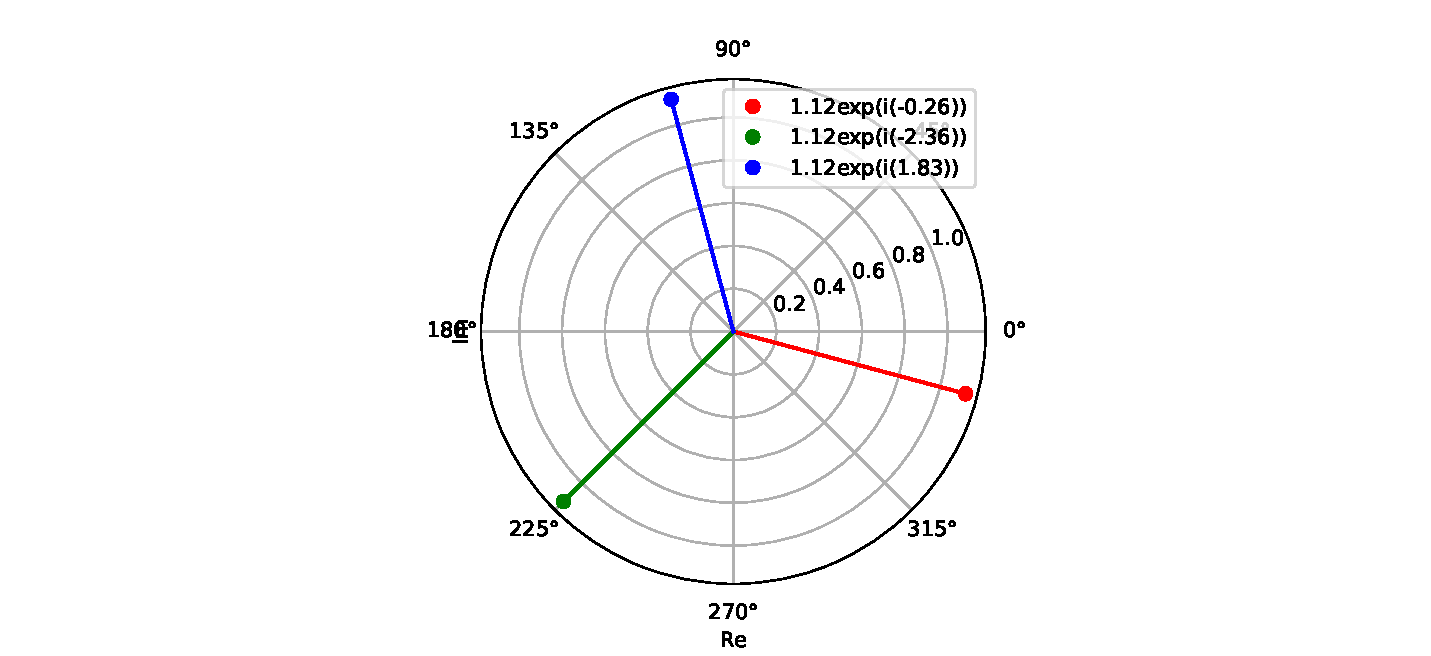
\includegraphics[scale=0.6]{13.2.21.pdf}
  \]
\end{oppgave}
\begin{oppgave}[25]
  Finner først $z=1-i$ på polar form.
  \[
    z = e^{i\pi/2}
  \]
  Ved De Moivres formel finner vi fjerderøttene
  \[
    \sqrt[4]{i} = \exp \left[\left(\frac{\pi}{8}+\frac{2\pi k}{4}\right)i\right], k\in\{0, 1, 2\}
  \]
  Kan plotte disse røttene i det komplekse plan:
  \[
    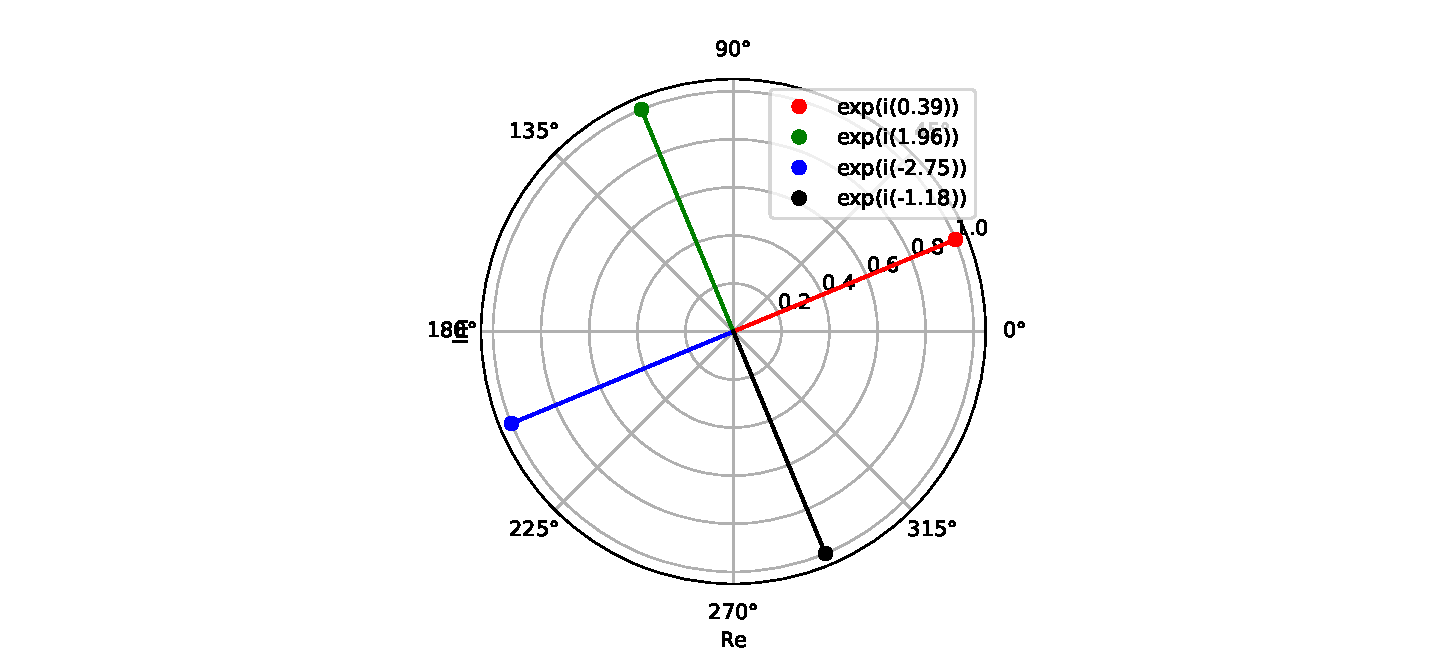
\includegraphics[scale=0.6]{13.2.25.pdf}
  \]
\end{oppgave}
\newpage
\section*{13.3}
\begin{oppgave}[6]
  Skriver om
  \[
    \text{Re}(1/z) = \frac{x}{x^2+y^2} \Rightarrow x>x^2+y^2
  \]
  Ser at vi kan skrive dette om til
  \[
    (x-1/2)^2+y^2>(1/2)^2
  \]
  Dermed tilsvarer det oppgitte området det komplekse planet ekskludert en sirkel med radius 0.5, med senter i (1,0).
\end{oppgave}
\begin{oppgave}[15]
  Forenkler uttrykket
  \[
    |z^2|\text{Im}(1/z)=(x^2+y^2)\frac{-y}{x^2+y^2} = -y
  \]
  Ser tydelig att dette vil gå mot null i origo, slik at funksjonen er kontinuerlig.
\end{oppgave}
\begin{oppgave}[16]
  Forenkler til
  \[
    \frac{\text{Im}(z)^2}{|z|^2} = \frac{r^2\sin(2\theta)}{r^2}=\sin(2\theta)
  \]
  Ser at denne grenseverdien ikke er veldefinert når $r\rightarrow 0$, slik at funksjonen ikke er kontinuerlig.
\end{oppgave}
\begin{oppgave}[18]
  Vil finner den deriverte til
  \[
    f(z)=\frac{z-i}{z+i}
  \]
  Bruker kjente derivasjonsregler, som gir
  \[
    f'(z)=\frac{(z+i)-(z-i)}{(z+i)^2} = \frac{2i}{(z+i)^2}
  \]
  Evaluerer dette i $z=i$:
  \[
    f'(i) = \frac{2i}{(2i)^2} = -\frac{i}{2}
  \]
  
\end{oppgave}
\end{document}